\section{Orchestration Algorithm}

\mnote{Usefulness evaluation}
In \autoref{chap:orchestration:algorithm}, we have proposed an application algorithm for transformation networks, which is proven correct, i.e., which returns only consistent models and does always terminate.
Thus, it conservatively approximates the orchestration problem.
We have motivated the strategy with its assistance in finding the reasons whenever it fails to deliver consistent models.
Since this property is difficult to prove, we provide an evaluation in the following.

\subsection{Goals and Methodology}
\label{chap:correctness_evaluation:orchestration:goals}

\mnote{Recapture algorithm}
The proposed provenance algorithm (see \autoref{algo:orchestration:provenance}) iteratively achieves consistency for subsets of the transformations.
This is based on the idea that if the algorithm fails, we know that all but the last executed transformation were executed in an order that yields consistent models and only the last executed transformation introduced some decision such that no consistent orchestration could be found anymore.

\begin{table}
    \renewcommand{\arraystretch}{1.4}
    \rowcolors{0}{\secondlinecolor}{\firstlinecolor}
    \begin{tabular}{L{8.2em} L{20em}}
        \toprule
        \rowcolor{\headinglinecolor}
        \goal{Orchestration} & 
            Show that the orchestration strategy helps transformation developers to find the cause for a transformation network not being able to find a consistent orchestration.\\
        \question[eq:orchestration:usefulness]{Usefulness} & 
            \questiontext{How far does the provenance algorithm improve the ability of identifying the reasons for a network not being able to find a consistent orchestration regarding an arbitrary strategy?} \\
        \metric &
            \metrictext{Considered transformations ratio: Ratio between the number of transformations to consider for finding a fault and the total number of transformations} \\
        \bottomrule
    \end{tabular}
    \caption[Goals, questions, metrics for orchestration]{Goals, questions and metrics for orchestration evaluation.}
    \label{tab:correctness_evaluation:gqm_orchestration}
\end{table}

\mnote{Evaluation goal and requirements}
We define the goal of our evaluation to show that the strategy helps transformation developers in finding the cause for a transformation network not to be able to find a consistent orchestration together with an according evaluation question and metric in \autoref{tab:correctness_evaluation:gqm_orchestration}.
For meaningful results, evaluation scenarios need to comprise more than three metamodels.
Failures especially occur due to cycles in the graph of transformations and since a setting with three metamodels contains at most one cycle, there is no real value in the proposed orchestration strategy.
Like we have discussed for the case studies in \autoref{chap:correctness_evaluation:categorization}, such scenarios are difficult to find.

\mnote{Controlled experiment}
Most meaningful results for this goal and question could be achieved with a controlled experiment, in which participants are confronted with the information provided by the proposed strategy for a set of scenarios in which it fails, as well as a control group to which the information delivered by other orchestration strategies is provided.
Then, metrics like the time or the number of steps required to find the reasons for the transformation networks to fail could be measured and compared.
Additionally, qualitative statements from interviews could be evaluated.

\mnote{Scenario-based discussion}
Since such an empirical evaluation requires high effort and, in particular, due to the absence of transformation networks to base the evaluation one, we decided not to perform such an empirical evaluation.
Instead, we provide a scenario-based discussion that exemplarily shows the benefits of the proposed strategy in two defined but not yet implemented scenarios.
We discuss two transformation networks with exemplary changes and how failures manifest with the proposed as well as alternative strategies and how this relates to the ability of identifying the reason for the failure.
This allows us to evaluate the usefulness of the strategy in terms of \autoref{eq:orchestration:usefulness} by measuring how many transformations have to be considered to identify a fault, according to the following metric:
\begin{align*}
    \mathvariable{considered\ transformations\ ratio = \frac{\#\ of\ transformations\ to\ consider%\ for\ identifying\ fault
    }{\#\ of\ total\ transformations}}
\end{align*}


\subsection{Scenarios}

\mnote{Two example scenarios}
We consider two scenarios of transformations and changes to existing models that are to be kept consistent by the transformations.
They represent extensions of scenarios that we already considered within the last chapters.
In both scenarios, our proposed strategy fails.
In one scenario, no consistent orchestration can be found because of incompatible consistency relations.
The other scenario contains a consistent orchestration. It may, however, take an arbitrarily long time to find it and no algorithm that is guaranteed to terminate can find it.


\subsubsection*{Incompatible Consistency Relations}

\begin{figure}
    \centering
    \newcommand{\hdistance}{19em}
\newcommand{\vdistance}{9em}
\newcommand{\classwidth}{6.8em}
\newcommand{\labeldistance}{1.0em}
\newcommand{\mmborder}{1em}

\begin{tikzpicture}[
    relation/.style={consistency relation, font=\footnotesize}
]

\pgfdeclarelayer{bg}
\pgfsetlayers{bg,main}

\umlclassvarwidth{pcm_component}{}{BasicComponent\sameheight}{
entityName
}{\classwidth}

\umlclassvarwidth[,right=\hdistance of pcm_component.north, anchor=north]{uml_class}{}{Class\sameheight}{
name
}{\classwidth}

\umlclassvarwidth[,below=\vdistance of pcm_component.north, anchor=north]{uml_component}{}{Component\sameheight}{
name
}{\classwidth}

\umlclassvarwidth[,right=\hdistance of uml_component.north, anchor=north]{java_class}{}{Class\sameheight}{
name
}{\classwidth}

\coordinate (pcm_label_coordinate) at ([yshift=\labeldistance]pcm_component.north);
\node[mmlabel, anchor=center] (pcm_label) at (pcm_label_coordinate) {\acrshort{PCM}};

\coordinate (uml_class_label_coordinate) at ([yshift=\labeldistance]uml_class.north);
\node[mmlabel, anchor=center] (uml_class_label) at (uml_class_label_coordinate) {\acrshort{UML} Class};

\coordinate (java_label_coordinate) at ([yshift=-\labeldistance]java_class.south);
\node[mmlabel, anchor=center] (java_label) at (java_label_coordinate) {Java};

\coordinate (uml_comp_label_coordinate) at ([yshift=-\labeldistance]uml_component.south);
\node[mmlabel, anchor=center] (uml_comp_label) at (uml_comp_label_coordinate) {\acrshort{UML} Component};

\begin{pgfonlayer}{bg}
    \node[mmbg, fit=(pcm_component)(pcm_label.center), inner sep=\mmborder] (pcm) {};
    \node[mmbg, fit=(java_class)(java_label.center), inner sep=\mmborder] (java) {};
    \node[mmbg, fit=(uml_class)(uml_class_label.center), inner sep=\mmborder] (uml_classes) {};
    \node[mmbg, fit=(uml_component)(uml_comp_label.center), inner sep=\mmborder] (uml_comp) {};
\end{pgfonlayer}

% CONSISTENCY RELATIONS
\draw[relation] (pcm_component.east) -- node[pos=0, below right] {$\mathvariable{bc}$} node[above ,align=center] {
    $\{\tupled{\mathvariable{bc}, \mathvariable{cl}} \mid$\\
    $\mathvariable{bc.entityName} = \mathvariable{cl.name}\}$
} node[pos=1, below left] {$\mathvariable{cl}$} (uml_class.west);
\draw[relation] (pcm_component.south) -- node[pos=0, below right] {$\mathvariable{bc}$} node[left, align=center] {
    $\{\tupled{\mathvariable{bc}, \mathvariable{co}} \mid$\\
    $\mathvariable{bc.entityName}$\\
    $= \mathvariable{co.name}\}$
} node[pos=1, above right] {$\mathvariable{co}$} (uml_component.north);
\draw[relation] (uml_component.east) -- node[pos=0, above right] {$\mathvariable{co}$} node[below] {$\setted{\tupled{\mathvariable{co}, \mathvariable{cl}} \mid \mathvariable{co.name} = \mathvariable{cl.name}}$} node[pos=1, above left] {$\mathvariable{cl}$} (java_class.west);
\draw[relation] (uml_class.south) -- node[pos=0, below left] {$\mathvariable{ucl}$} node[right, align=center] {
    $\{\tupled{\mathvariable{ucl}, \mathvariable{jcl}} \mid$\\
    $\mathvariable{ucl.name}$\\
    $= \mathvariable{jcl.name}\}$
} node[pos=1, above left] {$\mathvariable{jcl}$} (java_class.north);
\draw[relation] (uml_component) -- node[pos=0, above left=0em and -0.2em] {$\mathvariable{co}$} node[anchor=center, sloped, align=center] {
    $\{\tupled{\mathvariable{co}, \mathvariable{cl}} \mid$\\[0.3em]
    $\mathvariable{co.name} + "\mathvariable{Impl}" = \mathvariable{cl.name}\}$
} node[pos=1, below] {$\mathvariable{cl}$} (uml_class);

\end{tikzpicture}
    %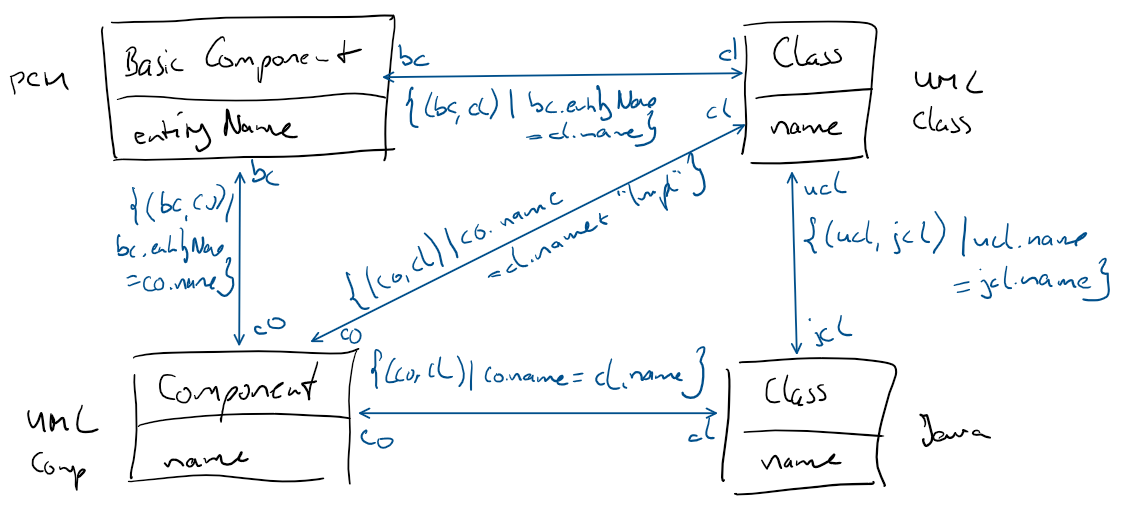
\includegraphics[width=\textwidth]{figures/correctness/evaluation/orchestration_scenario_cbse.png}
    \caption[Example scenario with incompatibility]{Consistency relations between basic components in \gls{PCM} model, components in \gls{UML} component models, classes in \gls{UML} class models and classes in Java models.}
    \label{fig:correctness_evaluation:orchestration:scenario_cbse}
\end{figure}

\mnote{Scenario description}
We depict the first scenario in \autoref{fig:correctness_evaluation:orchestration:scenario_cbse}.
It consists of consistency relations between different representations of software components and their realizing classes.
It comprises components in \gls{PCM} and \gls{UML}, as well as classes in \gls{UML} and Java.
The consistency relations between them describe a simple one-to-one mapping of their names, such that for each class and component the according other elements with the same name need to exist.
This is a simplification of the scenario that components have to be represented by classes, but not vice versa.
The only derivation from this mapping is the relation between \gls{UML} class and \gls{UML} component models, in which the class is specified to have the component name with an \enquote{Impl} suffix, according to the pattern proposed by \textcite{langhammer2017a}.

\mnote{Reasons for failing}
Independent from the actual realization of consistency preservation rules that try to preserve consistency according to these relations, any application algorithm for those transformations will fail because the relations are incompatible.
In fact, the induced set of consistent model tuples contains only the empty models, as the relations cannot be fulfilled by any instances of the depicted classes.
In consequence, adding any of the elements to a model will lead to an application algorithm that fails by either returning $\bot$, by returning inconsistent models, or by non-termination.
While not terminating, either the \enquote{Impl} suffix is repeatedly added and removed from the elements to locally fulfill the individual consistency relations, or the suffix is repeatedly appended to newly created elements, leading to an infinite number of elements with arbitrary long names.

\mnote{Distinction of failure cases}
When failing, an application algorithm can be in an arbitrary execution state, in which any of the models can be inconsistent.
The states in which the proposed provenance algorithm can fail can be divided into two categories.
\begin{longenumerate}
    \item If the first execution of the transformation between \gls{UML} class and \gls{UML} component models closes a cycle, i.e., two of the other transformations have already been executed such that the three form a cycle, the algorithm fails when adding that transformation.
    All transformations that were executed in advance are able to preserve consistency between all models, as they fulfill the consistency relations by adding the appropriate elements.
    When adding the transformation between \gls{UML} class and component models, the transformations cannot find a consistent tuple of models anymore, due to the incompatibility of their consistency relations.
    \item If the first execution of the transformation between \gls{UML} class and component models does not close a cycle, e.g., because after adding a \gls{UML} component it is the first transformation to be executed, or because only the transformation between \gls{UML} component models and \gls{PCM} component models and/or the one between \gls{UML} component models and Java code has been executed yet.
    Then the algorithm fails as soon as another transformation is executed that closes a cycle, such as the transformation between \gls{PCM} component models and \gls{UML} class model.
\end{longenumerate}
In either case, the algorithm fails as soon as the execution of transformations closes a cycle involving the transformation between \gls{UML} class and component models.
This does not necessarily mean that there is a fault in that transformation, but that there is a fault within one of the transformations in the cycle closed by the added transformation, as consistency to all other transformations could be preserved.
In fact, it is even impossible to say which transformation contains a fault, because it is even unclear whether the consistency relation between \gls{UML} class and component models is actually the one that should be adapted, or whether, for example, the ones between \gls{PCM} component models and \gls{UML} class models and between \gls{UML} component models and Java code should be adapted.

\mnote{Information for developer}
When the algorithm fails, the developer gets the information which addition of a transformation led to the failure and, in addition, the state of the models in which the algorithm aborted.
There is at least one consistency relation that is violated, which led to the abortion of the algorithm, and this consistency relation must belong to one of the transformations within the cycle containing the fault.
In consequence, the transformation developer must only consider the transformations in that cycle for finding the fault and, since he or she knows which consistency relation was violated, can restrict his- or herself to the elements concerned with the violated consistency relation.
While in this example each metamodel pair only shares one consistency relation, in larger transformations more relations may be involved.

\mnote{Number of considered transformations}
Regarding the number of transformations to consider for finding the fault, this means that at most three transformations need to be considered, as this is the largest simple cycle of transformations containing an incompatibility in its consistency relations:
\begin{align*}
    \mathvariable{considered\ transformations\ ratio} = \frac{3}{5}
\end{align*}
Even if the transformation between \gls{UML} class and component models is the last to be executed, still only three and not all five transformations need to be considered.
Although there is an incompatibility in both simple cycles in which that transformation is contained, investigating one is sufficient, because the fault must be visible in both of the simple cycles involving the last executed transformation.
Otherwise, the symmetric difference of the transformations in both cycles, which again forms a simple cycle, would also contain incompatible consistency relations.
This can, however, not be the case, as consistency to these transformations was already achieved before.
In the example, if the cycle of transformations between \gls{UML} component models, \gls{UML} class models and Java code did not contain an incompatibility, either the consistency relation between \gls{UML} component models and Java code or the one between \gls{UML} class models and Java code would need to assume the \enquote{Impl} suffix as well. Then, however, the cycle of relations between all four metamodels would contain an incompatibility as well.
% In general, if $\transformationset{T}_{\mathvariable{executed}} = \transformation{t}{1}, \dots, \transformation{t}{k}$ were executed and preserved consistency to all involved models and if adding a transformation $\transformation{t}{}$ then leads to a failure because of incompatible consistency relations, then any simple cycle of transformations in $\transformationset{T}_{\mathvariable{executed}} \cup \setted{\transformation{t}{}}$ in which $\transformation{t}{}$ is contained must contain incompatible consistency relations.
% If two cycles  and if $\transformation{t}{}$ forms at least two simple cycles with transformations in $\transformationset{T}_{\mathvariable{executed}}$
%Can be part of multiple cycles, but then it is problematic with both, because otherwise the cycle formed by the two cycles would be a problem as well (symmetric difference of transformations sets).

%Scenario 1:
%Es ist nicht klar, welche Transformation ursächlich ist. Ein Zyklus weist Probleme auf, aber ob die beiden ohne Impl oder die mit Impl "falsch" sind, ist unklar, aber auch nicht relevant.

%Only cycles containing the added transformation need to be considered


\subsubsection*{Orchestration Problem}

\begin{figure}
    \centering
    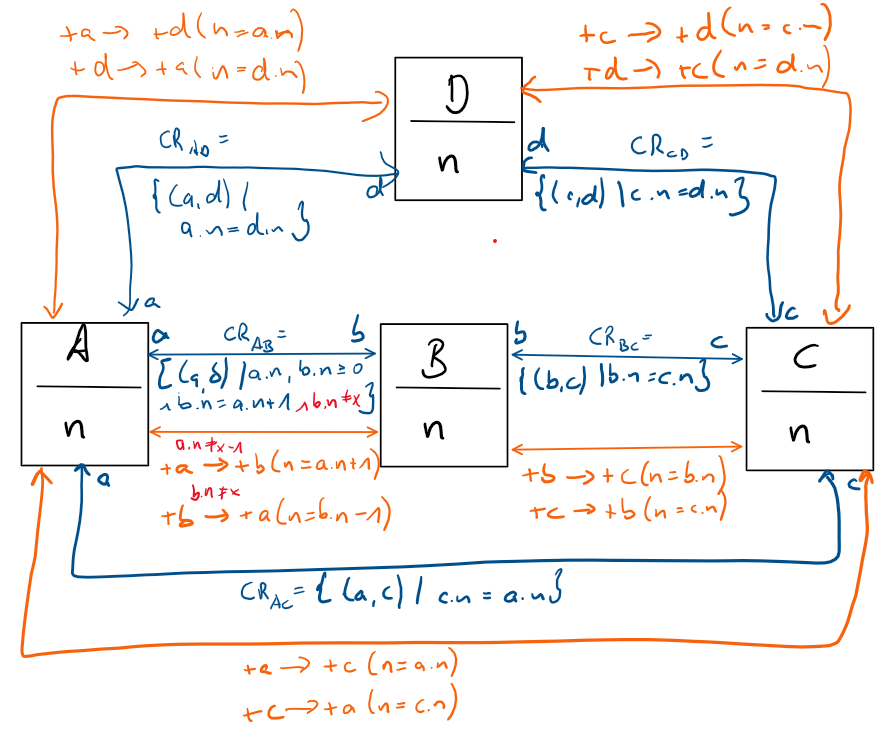
\includegraphics[width=\textwidth]{figures/correctness/evaluation/orchestration_scenario_counting.png}
    \caption[Example scenario with arbitrary execution bound]{Extension of the example in \autoref{fig:orchestration:no_upper_bound} with consistency relations that require an arbitrary number of transformation execution, depending on value $x$.}
    \label{fig:correctness_evaluation:orchestration:scenario_counting}
\end{figure}

\mnote{Scenario description}
\autoref{fig:correctness_evaluation:orchestration:scenario_counting} depictes the second scenario.
It is an extension of the abstract example depicted in \autoref{fig:orchestration:no_upper_bound} as a demonstration for the non-existence of an upper bound for the number of necessary transformation executions in a transformation network.
The extended example contains an additional metamodel, thus consisting of four metamodels, each containing one \metaclass. 
Apart from that, it also contains consistency relations that require for each of the abstract elements \texttt{A}, \texttt{B}, \texttt{C} and \texttt{D} other elements with the same value of $n$ to exist.
Only the relation between \texttt{A} and \texttt{B} requires the value $n$ of \texttt{B} to be higher by one than the one of \texttt{A}, except for some value $x$ of $n$, for which there must be no such element \texttt{B} for an existing \texttt{A}.
Although these constraints make it difficult to find consistent models, they are actually compatible, as for each element there is a consistent model tuple containing it.

\mnote{Reasons for failing}
The depicted consistency preservation rules try to resolve this issue by adding elements to fulfill the consistency relations.
This leads to the situation that adding an element \texttt{A} with value $1$ at least $x-1$ transformation executions are necessary (see \autoref{lemma:minimal_executions}).
Thus, any application algorithm must either perform that many executions or fail returning $\bot$ or inconsistent models.
When an algorithm performs that many executions, it can actually not be allowed to define any arbitrary execution bound because the value of $x$ can be arbitrarily high.
Thus due to the orchestration problem, as discussed in \autoref{chap:orchestration:decidability:algorithm}, such a behavior leads to non-termination in other scenarios, which is not a competitive behavior compared to our proposed algorithm, since we want to avoid non-termination.
In consequence, any useful application algorithm will fail in that example.

\mnote{Number of considered transformations}
While an arbitrary application algorithm with an artificial termination criterion will fail in an unexpected state without any guarantee for usefulness of the state in which it fails to identify the reason for the failure, the provenance algorithm fails in the same cases and in the same way that we have already discussed for the first scenario.
As soon as a transformation is executed that induces a cycles with the executed ones and contains the transformation between \texttt{A} and \texttt{B}, the algorithm will fail.
In that case, the developer knows that the problem arises from the transformations in the cycle that was closed by the last executed transformation.
This improves the process of finding the cause for the failure in the way as in the first example.
In the worst case, the first cycle closed during execution containing the transformation between \texttt{A} and \texttt{B} is the one of length $4$ between all metamodels.
Thus, we have:
\begin{align*}
    \mathvariable{considered\ transformations\ ratio} = \frac{4}{5}
\end{align*}


\subsection{Discussion and Validity}
\label{chap:correctness_evaluation:orchestration:discussion}

The discussed scenarios give us specific insights about the usefulness of the proposed provenance algorithm, which we summarize in the following.
In addition, we discuss threats to the validity of the results that especially arise from the construction of our scenario-based evaluation.

\subsubsection{Insights}

\mnote{General restriction considered transformations}
In the discussed scenarios, we have seen that using the provenance algorithm the number of transformations to consider for finding a fault that leads to a failure during execution is restricted by the length of the largest simple cycle of transformations that contains the faulty transformation.
By construction of the algorithm, it fails as soon as a cycle of executed transformations is closed that contains a faulty one.
In addition, by construction the fault can be found in each of the simple cycles of the already executed transformations that contain the last executed one.
Thus, in the worst case the transformations in the largest simple cycle of transformations containing the faulty one need to be considered.
In consequence, as long as the transformation network does not only consist of one simple cycle of transformations, the algorithm does always ensure that not all transformations need to be considered in case of a failure.
In fact, it ensures that in a network of $n$ metamodels at most $n$ transformations need to be considered.

\mnote{Transformation selection order}
This also shows that we can further improve the algorithm by determining a reasonable selection order for the transformations.
Rather than choosing an arbitrary transformation to be executed next, cycles should be closed first, because this ensures that smaller simple cycles are closed early.
As an example, consider the second scenario.
If we first execute the transformation between \texttt{A} and \texttt{B} and then the one between \texttt{B} and \texttt{C}, it is better to then execute the one between \texttt{A} and \texttt{C} to close the cycle, as the algorithm then already fails.
If the transformations to \texttt{D} are executed before closing that cycle, we first close a cycle of length $4$ rather than one of length $3$. Both lead to a failure, but we expect the effort to find the fault in the latter case to be lower.

\mnote{Evidence of results}
Since we did not perform an empirical evaluation but only a scenario-based discussion, our finding only serve as an initial indicator for the usefulness of the provenance algorithm in terms of improving the ability to identify reasons for failing as asked by \autoref{eq:orchestration:usefulness}.
Still, we found a criterion in the scenarios that limits the number of transformations that need to be considered to identify a fault by construction of the algorithm, which is an improvement regarding any arbitrary other strategy, which, in the worst case, can require the investigation of all transformations.
Whether or not this metric reasonably reflects usefulness of the approach does, however, remain a threat to validity until its validation in an experiment.

%Could be beneficial to execute in different orders. This allows to identify the cycle. E.g., in first scenario, if problematic transformation is executed last, then unclear which of the two involved cycles is the problem. 

% To answer the question:
% - Only cycles containing the added transformation need to be considered
% - General statements regarding cycles generalize 
% - Number of considered transformations restricted by maximal length of simple cycle.

% Improvements by order


\subsubsection{Threats to Validity}

In the evaluation, we found a criterion that shows that the proposed algorithm improves the investigated metric in all cases.
Still, there are threats to construct and external validity that need to be mitigated by further studies.

\mnote{Construct validity}
We assumed the number of transformations to consider to be related to the usefulness of the strategy in terms of the ability to find a fault.
Whether this assumption holds is a threat to construct validity.
To mitigate this threat, we did not only focus on the evaluation of that metric but also presented qualitative arguments and discussed further quantifiable improvements, such as the restriction of consistency relations to consider in the failure case.

\mnote{External validity}
Finally, we have compared our proposed approach with an arbitrary strategy for transformation orchestration.
In this comparison, we always guarantee an improvement in worst-case performance.
There may, however, be another strategy that performs better or at least equal to the proposed approach in all cases.
This can limit external validity of the results.
We tried to mitigate this issue by systematically deriving a strategy for orchestration that performs better than other strategies in all cases with respect to a well-defined criterion.
As discussed in \autoref{chap:orchestration:conservative:improvement}, we developed a simulator for evaluating different strategies, but unfortunately we found each strategy to be outperformed by at least one other strategy regarding their the ability to find a consistency orchestration in at least one scenario.
Thus, we do not expect another strategy to be systematically better than the one we proposed, but, in the best case, only to perform better in specific situations.


\subsection{Limitations and Future Work}
\label{chap:correctness_evaluation:orchestration:limitations}

\paragraph{Evidence for Generalizability}
\mnote{Controlled experiment}
The most relevant limitation of the proposed algorithm concerns the validity of the evaluation results regarding the proposed properties of the approach.
While statements on the correctness and well-definedness of the approach have been proven, its usefulness was only validated in a scenario-based discussion, which especially suffers from potential threats to construct validity, as it is unclear whether the metric we have investigated actually reflect usefulness of the strategy in terms of reducing the time and effort when identifying faults in transformation networks.
Thus, in future work we plan to perform a controlled experiment in which the information delivered by our approach and by other strategies are presented to different groups of developers.
Evaluating how long they take to find and fix faults and how successful they are in both situations helps us to further validate the expected properties and improve evidence of the results.

\paragraph{Well-defined Design Property}
\mnote{Usefulness of design property}
The provenance algorithm gives the guarantee of finding a consistent orchestration as long as the transformations fulfill the property of being reactive converging (see \autoref{def:reactiveconverging}).
This property can, however, neither be easily guaranteed nor analyzed.
We have argued why this is still a reasonable property, but a property that can at least be analyzed at design time to avoid failures during execution would still be beneficial.
Such a property can, however, easily restrict expressiveness of transformations, as we have discussed in \autoref{chap:orchestration:decidability:restriction}.
Still, finding such a property would be a valuable contribution and thus serves as a starting point for future work.

\paragraph{Transformation Selection Order}
\mnote{Systematic execution order}
In the evaluation, we found that selecting transformations in an order such that smaller cycles of executed transformations are closed first may be beneficial, because it reduces the number of transformations that need to be investigated to find a fault whenever the algorithm fails.
While the considerations in the evaluation scenarios indicate it to be reasonable, we want to systematically investigate such an order and, in the best case, prove its improvement in future work.

\paragraph{Holistic Application Process}
\mnote{Fault identification process}
Finally, we have only discussed how our proposed approach supports a transformation developer in identifying faults in transformations.
In practice, a failure may however not occur when a transformation developer tests a transformation network, which allows him to directly identify and fix the fault.
Instead, a transformation network may be in productive use, thus a failure occurs when a user of that network applies the transformations to preserve consistency.
Then, a holistic process is required for reporting and fixing such errors, which needs to define the responsibilities.
Additionally, such a process will not be just-in-time, thus the project in which the transformation network is applied needs to be able to deal with the fact that consistency cannot be preserved for some time.
Such a process is, for example, also part of the research in the \vitruv project (see~\cite{klare2020Vitruv-JSS}), to which the results of this thesis contribute, and thus a general topic of future work.
The author of this thesis also contributed to a group discussion in a Dagstuhl seminar that considered that topic~\owncite{klare2019dagstuhl}.


% \subsubsection{Limitations}
% \label{chap:correctness_evaluation:orchestration:discussion:limitations}

% \mnote{Evidence for generalizability}
% The most relevant limitation of the proposed algorithm concern the validity of the evaluation results regarding the proposed properties of the approach.
% Thus, in future work, we plan to perform a controlled experiment to further validate the expected properties by investigating how the approach improves the process of identifying errors in transformation networks in terms of required time and steps (see \autoref{chap:futurework:correctness:orchestration:experiment}).

% \mnote{Usefulness of design property}
% The provenance algorithm gives the guarantee of finding a consistent orchestration as long as the transformations fulfill the property of being reactive converging (see \autoref{def:reactiveconverging}).
% This property can, however, neither be easily guaranteed nor analyzed.
% We have argued why this is still a reasonable property, but a property that can at least be analyzed at design time to avoid failures during execution would be still benefits.
% This is why we try to find such a property in future work, as discussed in \autoref{chap:futurework:correctness:orchestration:property}.

% \mnote{Transformation selection order}
% In the evaluation, we found that selecting transformations in an order such that smaller cycles of executed transformations are closed first.
% While the considerations in the evaluation scenarios indicate it to be reasonable, we want to systematically investigate such an order an, in the best case, prove its improvement in future work (see \autoref{chap:futurework:correctness:orchestration:selection}).

% \mnote{Holistic application process}
% Finally, we have only discussed how our proposed approach supports a transformation developer in identifying faults in transformations.
% It is, however, not clear how a holistic process has to look like, in which a failure may occur during the application of transformations in actual software development projects.
% Responsibilities for fixing a fault in such a situation and dealing with the delay between the fix and the proceeded development of the software project are not yet clear and need to be investigated in future work, as proposed in \autoref{chap:futurework:correctness:orchestration:process}.
% The author of this thesis contributed to a group discussion in a Dagstuhl seminar that considered that topic~\owncite{klare2019dagstuhl}.
